\documentclass[conference]{IEEEtran}
\IEEEoverridecommandlockouts

\usepackage{cite}
\usepackage{amsmath,amssymb}
\usepackage{graphicx}
\usepackage{booktabs}
\usepackage{array}
\usepackage{url}
\usepackage[hidelinks]{hyperref}

\graphicspath{{figs/}}

\begin{document}

\title{Capacity Scaling of YOLO26-OBB for Oriented Military
Aircraft Detection in Satellite Imagery: A Case Study on MAR20}

\author{
\IEEEauthorblockN{Author Name}
\IEEEauthorblockA{Affiliation\\
City, Country\\
email@example.com}
}

\maketitle

\begin{abstract}
Detecting and classifying individual military aircraft in overhead imagery requires
oriented bounding boxes (OBB): parked aircraft sit at arbitrary azimuths, and a
horizontal box conflates neighbouring airframes on a dense apron. We report a
controlled capacity study of the YOLO26-OBB detector family on the MAR20
benchmark, where twenty aircraft classes are annotated with oriented quadrilaterals.
Three backbone scales (nano, small, medium) are trained with an identical recipe at
$1024\times1024$ input with full $180^\circ$ rotation augmentation, differing only in
capacity; the medium-scale model is trained under two-GPU distributed data parallel.
Accuracy increases monotonically with capacity on every aggregate metric, reaching
mAP@0.5 of 0.916 and mAP@0.5:0.95 of 0.801 for the medium model, against 0.891/0.786
for small and 0.871/0.762 for nano. Per-class analysis shows that the gain is
concentrated in two recall-limited fighter classes, while the single precision-limited
class is unaffected by a doubling of parameters. We argue this separates two failure
modes that aggregate mAP hides: failing to \emph{find} a small airframe, which is
capacity-bound, and failing to \emph{identify} it, which is not. We also report
converged-window statistics alongside best-epoch figures, because the gap between the
two is large enough to change how the results should be read.
\end{abstract}

\begin{IEEEkeywords}
oriented object detection, remote sensing, aircraft recognition, YOLO, capacity
scaling, MAR20
\end{IEEEkeywords}

\section{Introduction}

Monitoring airbases from orbit is a routine remote-sensing task with applications in
fleet counting, activity assessment, and change detection. The interesting quantity is
rarely ``is there an aircraft'' but ``which aircraft, and how many of each''. That
makes the problem instance-level detection with fine-grained classification, on
targets that are small, densely packed, and viewed from directly above.

Two properties of this setting shape the design space. First, orientation is
informative and horizontal boxes discard it: a $50$~m bomber and a $15$~m fighter
rotated a few degrees can share a horizontal box, and adjacent aircraft in a row
overlap heavily under axis-aligned parameterisation. Oriented bounding boxes remove
both problems and additionally give a heading estimate, which is what an analyst
actually wants when reading a flight line. Second, the targets are small in absolute
terms. A fighter is roughly $48\times48$ pixels at a $1024$~px input, so the
discriminative signal available for classification is a few pixels of wing sweep and
tail arrangement.

Recent single-stage oriented detectors handle the geometry well, and the YOLO family
in its OBB variant has made them cheap to train and deploy. What is less well
documented is how accuracy responds to backbone capacity at a fixed, generous input
resolution, and whether the residual errors of such a detector are uniform across
classes or structurally concentrated. The second question matters more than the first
for anyone planning a deployment: a model whose remaining errors are all
detection failures can be helped by capacity, better augmentation, or a lower
operating threshold, whereas a model whose errors are identity confusions needs a
different intervention entirely.

This paper contributes:
\begin{itemize}
\item a controlled three-rung capacity ladder (nano, small, medium) for YOLO26-OBB on
MAR20, trained with a single identical recipe and identical augmentation, so that the
only free variable is backbone width;
\item a per-class analysis that resolves the aggregate gain into two distinct failure
modes, one of which is capacity-bound and one of which is not;
\item accuracy reporting that pairs best-epoch values with converged-window
statistics, and a discussion of why the former overstates performance under
early-stopping;
\item measured training throughput and inference latency for all three scales on the
same hardware.
\end{itemize}

The remainder is organised as follows. Section~\ref{sec:related} places the work
relative to oriented detection and to aircraft-recognition benchmarks.
Section~\ref{sec:method} describes the dataset, the detector, and the training recipe.
Section~\ref{sec:setup} states the experimental protocol.
Section~\ref{sec:results} reports results and the per-class analysis.
Section~\ref{sec:limits} discusses limitations, and Section~\ref{sec:concl}
concludes.

\section{Related Work}
\label{sec:related}

\subsection{Generic and oriented detection}
Two-stage and single-stage detectors with axis-aligned boxes are mature
\cite{redmon2016,lin2017focal,tian2019fcos,zhou2019objects}. Oriented detection
developed largely around aerial imagery, where the DOTA benchmark
\cite{xia2018dota} established the task and evaluation protocol. Rotated region
proposals \cite{ding2019roitransformer}, rotation-equivariant backbones
\cite{han2021redet}, and refined single-stage heads \cite{yang2021r3det} each address
a different part of the problem: proposal alignment, feature equivariance, and
iterative box refinement respectively. The YOLO-OBB variant takes the opposite
engineering direction: keep a single-stage anchor-free head and accept a coarser
angle estimate in exchange for a simple, fast pipeline. Removing non-maximum
suppression entirely, as recent end-to-end heads do, is particularly relevant here
because dense aprons produce hundreds of mutually overlapping oriented boxes, which
is exactly the regime where suppression cost dominates.

\subsection{Aircraft recognition in overhead imagery}
Fine-grained aircraft recognition has its own literature, driven by the difficulty of
separating planforms that differ by a few pixels at the available ground sample
distance. MAR20 \cite{yu2021mar20} is the reference benchmark for military aircraft:
twenty classes spanning US, Russian, and allied types, annotated with oriented boxes,
collected to stress exactly the fine-grained regime. Reported results on MAR20 are
typically high for large multi-engine airframes and substantially lower for
single-engine fighters, which is the pattern our per-class results reproduce and, we
argue, partly explain.

\subsection{Capacity scaling}
Compound scaling studies \cite{tan2019efficientnet} and speed--accuracy analyses of
detector families \cite{huang2017speed} established that accuracy is a smooth function
of capacity only within a regime; past some point the binding constraint shifts from
parameters to data, resolution, or label noise. Our ladder is designed to locate that
shift for one detector family on one dataset, rather than to maximise accuracy.

\section{Dataset and Method}
\label{sec:method}

\subsection{MAR20 and preprocessing}
MAR20 comprises 3{,}842 satellite images covering twenty military aircraft classes:
fighters (F-15, F-16, F-22, F/A-18, SU-24, SU-34, SU-35), bombers (B-1B, B-52, TU-22,
TU-95, TU-160), transports (C-5, C-17, C-130), tankers (KC-10, KC-135), airborne
early-warning aircraft (E-3, E-8), and maritime patrol (P-3C). Ground sample distance
varies across scenes in the $0.3$--$0.5$~m range, which makes apparent object size a
function of source scene as well as of aircraft type; this is one reason the benchmark
is harder than its nominal resolution suggests.

Annotations are oriented quadrilaterals in DOTA format. We convert them to the
normalised eight-coordinate representation expected by the OBB head and remap the
label indices to a fixed class order derived from the dataset configuration, so that
class identity is stable across runs. The predefined split is used unmodified:
1{,}331 training images and 2{,}511 validation images, with no airfield shared between
the two. Instance counts are 7{,}870 and 14{,}471 respectively. The validation set is
nearly twice the training set; we treat this as a property of the benchmark's
predefined split rather than a choice.

\subsection{Detector}
We use YOLO26-OBB at three backbone scales. The head is anchor-free and
end-to-end: non-maximum suppression is removed, and distribution-focal-loss
regression is replaced with direct regression of box extent and rotation angle. For
our setting both changes are operationally relevant. Removing suppression matters
because dense rows of aircraft are precisely the case where suppression either costs
time or, if made aggressive, deletes true positives. Direct angle regression is
cheaper to train than a discretised angle distribution but gives a coarser heading
estimate, which we accept: heading is a by-product of this work, not its objective.

\subsection{Training recipe}
All three runs use one recipe, and differ only in the checkpoint that initialises
training and in the number of GPUs used. Input resolution is $1024\times1024$;
batch size is 32 in total; images are cached in RAM, removing per-epoch decode;
mixed precision is enabled; the optimiser is selected automatically with an initial
learning rate of 0.01 under a cosine schedule and three warmup epochs; the epoch
budget is 200 with early stopping at a patience of 60 epochs on validation fitness;
and mosaic is disabled for the final ten epochs so the model finishes on unaugmented
geometry. Determinism is requested (fixed seed, deterministic kernels), which gives
run-to-run stability on one device but not across devices (Section~\ref{sec:limits}).

The one augmentation decision that is specific to this task is rotation. Because
satellite azimuth is arbitrary and unrelated to the aircraft heading, we enable full
$180^\circ$ rotation rather than the small-angle jitter typical of ground-level
detection. Combined with horizontal flips, mosaic, and standard photometric
augmentation, this makes the training distribution approximately invariant to the
symmetry the task actually has. Flipping vertically was left off as it duplicates
the horizontal flip under $180^\circ$ rotation.

\section{Experimental Protocol}
\label{sec:setup}

\subsection{Hardware}
The nano and small runs each used a single NVIDIA L40S (48~GB). The medium run used
two L40S cards under distributed data parallel with 16 images per card, so the total
batch seen by the optimiser is unchanged but gradients are averaged across devices.

\subsection{Metrics}
We report standard detection metrics at IoU 0.5 and averaged over 0.5:0.95, together
with precision and recall at the default operating point, in all cases class-averaged
over the twenty classes. Because every run early-stopped and reports the checkpoint
selected on the same validation split, we additionally report a
\emph{converged level}: the mean and standard deviation of the metric over the final
60 epochs of each run. This is the more honest estimator of what a retrained model of
the same configuration would deliver, since best-epoch selection is a maximum taken
over exactly the epoch-to-epoch jitter the level quantifies.

Latency is measured per image at batch size 1 on the training card, split into
preprocessing, inference, and postprocessing. It is a datacenter-GPU number and is
not a deployment figure.

\subsection{Reproducibility}
Every run is launched from the same script with the checkpoint and run name as the
only varying arguments; the resolved hyperparameters are dumped into each run
directory alongside the per-epoch metrics, so the recipe is auditable rather than
asserted. Reported metrics are taken from a standalone validation pass over the full
2{,}511-image split, separate from the training loop, and agree with the training
log to the printed precision.

\section{Results and Discussion}
\label{sec:results}

\begin{table}[t]
\centering
\caption{Capacity ladder. All runs share one recipe at $1024$~px with
$180^\circ$ rotation augmentation. ``Peak'' is the selected best epoch;
``level'' is the mean over the final 60 epochs of the run. Parameter counts are
pre-folding; the batch-norm-fused small model reports 9.76~M.}
\label{tab:ladder}
\setlength{\tabcolsep}{4pt}
\begin{tabular}{@{}lccc@{}}
\toprule
 & nano & small & medium \\
\midrule
Parameters (M) & 2.6 & 10.5 & 21.2 \\
Compute (GFLOPs) & -- & 21.8 & 71.9 \\
GPUs & 1 & 1 & 2 (DDP) \\
Epochs run / best & 168 / 108 & 160 / 100 & 102 / 42 \\
Train time (min) & 51 & 72 & 47 \\
Inference (ms) & -- & 4.0 & 9.5 \\
\midrule
mAP@0.5 (peak) & 0.871 & 0.891 & \textbf{0.916} \\
mAP@0.5:0.95 (peak) & 0.762 & 0.786 & \textbf{0.801} \\
Precision (peak) & 0.826 & 0.864 & \textbf{0.889} \\
Recall (peak) & 0.822 & 0.842 & \textbf{0.859} \\
\midrule
mAP@0.5 (level) & 0.853 & 0.866 & \textbf{0.889} \\
mAP@0.5:0.95 (level) & 0.747 & 0.763 & \textbf{0.779} \\
Level std (mAP@0.5) & 0.004 & 0.009 & 0.014 \\
Epochs $\geq 0.90$ & 0 & 0 & 17 \\
\bottomrule
\end{tabular}
\end{table}

\subsection{Aggregate behaviour}
Table~\ref{tab:ladder} summarises the three runs. Accuracy is monotonic in capacity
on every aggregate metric, and no rung trades one metric for another: nano to small,
a fourfold increase in parameters, buys $+0.0206$ mAP@0.5 and $+0.0242$ mAP@0.5:0.95
together with $+0.038$ precision and $+0.020$ recall; small to medium, a doubling,
buys a further $+0.0246$ and $+0.0141$. Measured on the converged level instead, the
steps are $+0.013$/$+0.016$ and $+0.023$/$+0.016$ respectively. Both readings agree in
sign and order of magnitude, and each step exceeds the epoch-to-epoch spread of the
larger of the two runs it compares, so the ordering is not an artefact of noise; with
one run per scale, however, each step is a single observation rather than a
distribution. The
medium run is also the first configuration to cross 0.90 mAP@0.5 as a stable level
rather than as a single epoch: 17 of its 102 epochs sit at or above 0.90.

The monotonicity has a direct interpretation. At $1024$~px, accuracy in this regime is
still capacity-bound rather than resolution-bound: the same pixels support a better
model, and the medium run improves without any change to input size or augmentation.
For a deployment with a compute budget, that means the resolution has already been
spent well and the remaining trade is parameter count against latency.

\subsection{Where the gain comes from}

\begin{table}[t]
\centering
\caption{Per-class mAP@0.5 for the small and medium models on the 2{,}511-image
validation split. Instances are validation instances. Rows sorted by medium-model
accuracy.}
\label{tab:perclass}
\setlength{\tabcolsep}{4pt}
\begin{tabular}{@{}lcccccc@{}}
\toprule
Class & small & medium & $\Delta$ & $P$ & $R$ & Inst. \\
\midrule
B-52   & 0.987 & 0.992 & $+0.005$ & 0.947 & 0.971 & 579 \\
B-1B   & 0.986 & 0.989 & $+0.003$ & 0.921 & 0.991 & 556 \\
TU-95  & 0.955 & 0.988 & $+0.033$ & 0.944 & 0.984 & 958 \\
C-17   & 0.986 & 0.986 & $\pm0.000$ & 0.961 & 0.950 & 860 \\
C-130  & 0.981 & 0.981 & $\pm0.000$ & 0.984 & 0.919 & 993 \\
TU-160 & 0.969 & 0.978 & $+0.009$ & 0.981 & 0.920 & 334 \\
C-5    & 0.970 & 0.976 & $+0.006$ & 0.979 & 0.924 & 463 \\
P-3C   & 0.968 & 0.975 & $+0.007$ & 0.964 & 0.926 & 611 \\
F/A-18 & 0.840 & 0.953 & $+0.113$ & 0.986 & 0.731 & 1847 \\
E-3    & 0.980 & 0.950 & $-0.030$ & 0.824 & 0.994 & 489 \\
TU-22  & 0.936 & 0.945 & $+0.009$ & 0.750 & 0.957 & 462 \\
SU-35  & 0.914 & 0.944 & $+0.030$ & 0.917 & 0.870 & 1092 \\
KC-135 & 0.925 & 0.944 & $+0.019$ & 0.945 & 0.834 & 1119 \\
SU-34  & 0.851 & 0.900 & $+0.049$ & 0.922 & 0.752 & 717 \\
SU-24  & 0.927 & 0.868 & $-0.059$ & 0.980 & 0.706 & 551 \\
E-8    & 0.847 & 0.866 & $+0.019$ & 0.784 & 0.794 & 356 \\
F-15   & 0.617 & 0.851 & $+0.234$ & 0.906 & 0.750 & 1091 \\
F-16   & 0.821 & 0.840 & $+0.019$ & 0.813 & 0.763 & 827 \\
KC-10  & 0.774 & 0.777 & $+0.003$ & 0.809 & 0.723 & 148 \\
F-22   & 0.600 & 0.615 & $+0.015$ & 0.451 & 0.742 & 418 \\
\bottomrule
\end{tabular}
\end{table}

Table~\ref{tab:perclass} shows that the aggregate $+0.025$ is not spread across the
class set. Fifteen of the twenty classes move by $0.03$ or less; the large
multi-engine airframes are saturated at $0.98$--$0.99$ under both scales; and nearly
the entire gain is carried by two fighter classes, F-15 ($0.617\rightarrow0.851$,
$+0.234$) and F/A-18 ($0.840\rightarrow0.953$, $+0.113$). The mean over the four
fighter classes rises from $0.720$ to $0.815$ while the mean over the remaining
sixteen moves from $0.935$ to $0.941$. Doubling the backbone bought fighter-class
recall and almost nothing else.

This matters because the two improved classes and the one unchanged class fail in
opposite ways. On the small model, F-15 had precision 0.723 with recall 0.521 and
F/A-18 had precision 0.974 with recall 0.556: both were confident when they fired and
simply failed to fire often enough. The medium model lifts F-15 to 0.906/0.750 and
F/A-18 to 0.986/0.731, i.e.\ it repairs the recall deficit directly, and F-15's
mAP@0.5:0.95 gain ($0.533\rightarrow0.735$), so the boxes are also better localised
rather than merely more numerous: both metrics improve by the same proportion
(about $38\%$), which is what one expects if localisation quality scales with the
number of correctly found instances.

F-22 behaves differently. It moves from 0.600 to 0.615, and its precision
\emph{falls} from 0.493 to 0.451 while recall rises from 0.687 to 0.742. More
capacity made it more willing to assert a class it cannot resolve: the additional
parameters buy detections that are then assigned to the wrong twin-tail fighter. This
is the signature of an identity limit rather than a detection limit. Consistent with
that, SU-24 loses $0.059$ through a recall drop ($0.877\rightarrow0.706$) with
precision rising to 0.980, and E-3 loses $0.030$ through precision
($0.939\rightarrow0.824$) with recall at 0.994. Both remain above 0.85, but the wider
model appears to shift some capacity away from these classes toward the fighters.

We therefore read the outcome as follows. The residual error of the small model is
\emph{two} phenomena, and aggregate mAP conflates them: failing to \emph{find} an
airframe, which is capacity-bound and was fixed by the medium backbone, and failing to
\emph{identify} it, which is not and was not. Class instance count is a weak predictor
of which case applies ($r=0.27$, $r^{2}=0.07$ across the twenty classes): F-22 has 418
validation instances and scores 0.615, while TU-160 has 334 and scores 0.978. What
separates them is the discriminability of the planform at this ground sample distance,
not the amount of supervision available.

\begin{figure}[t]
\centering
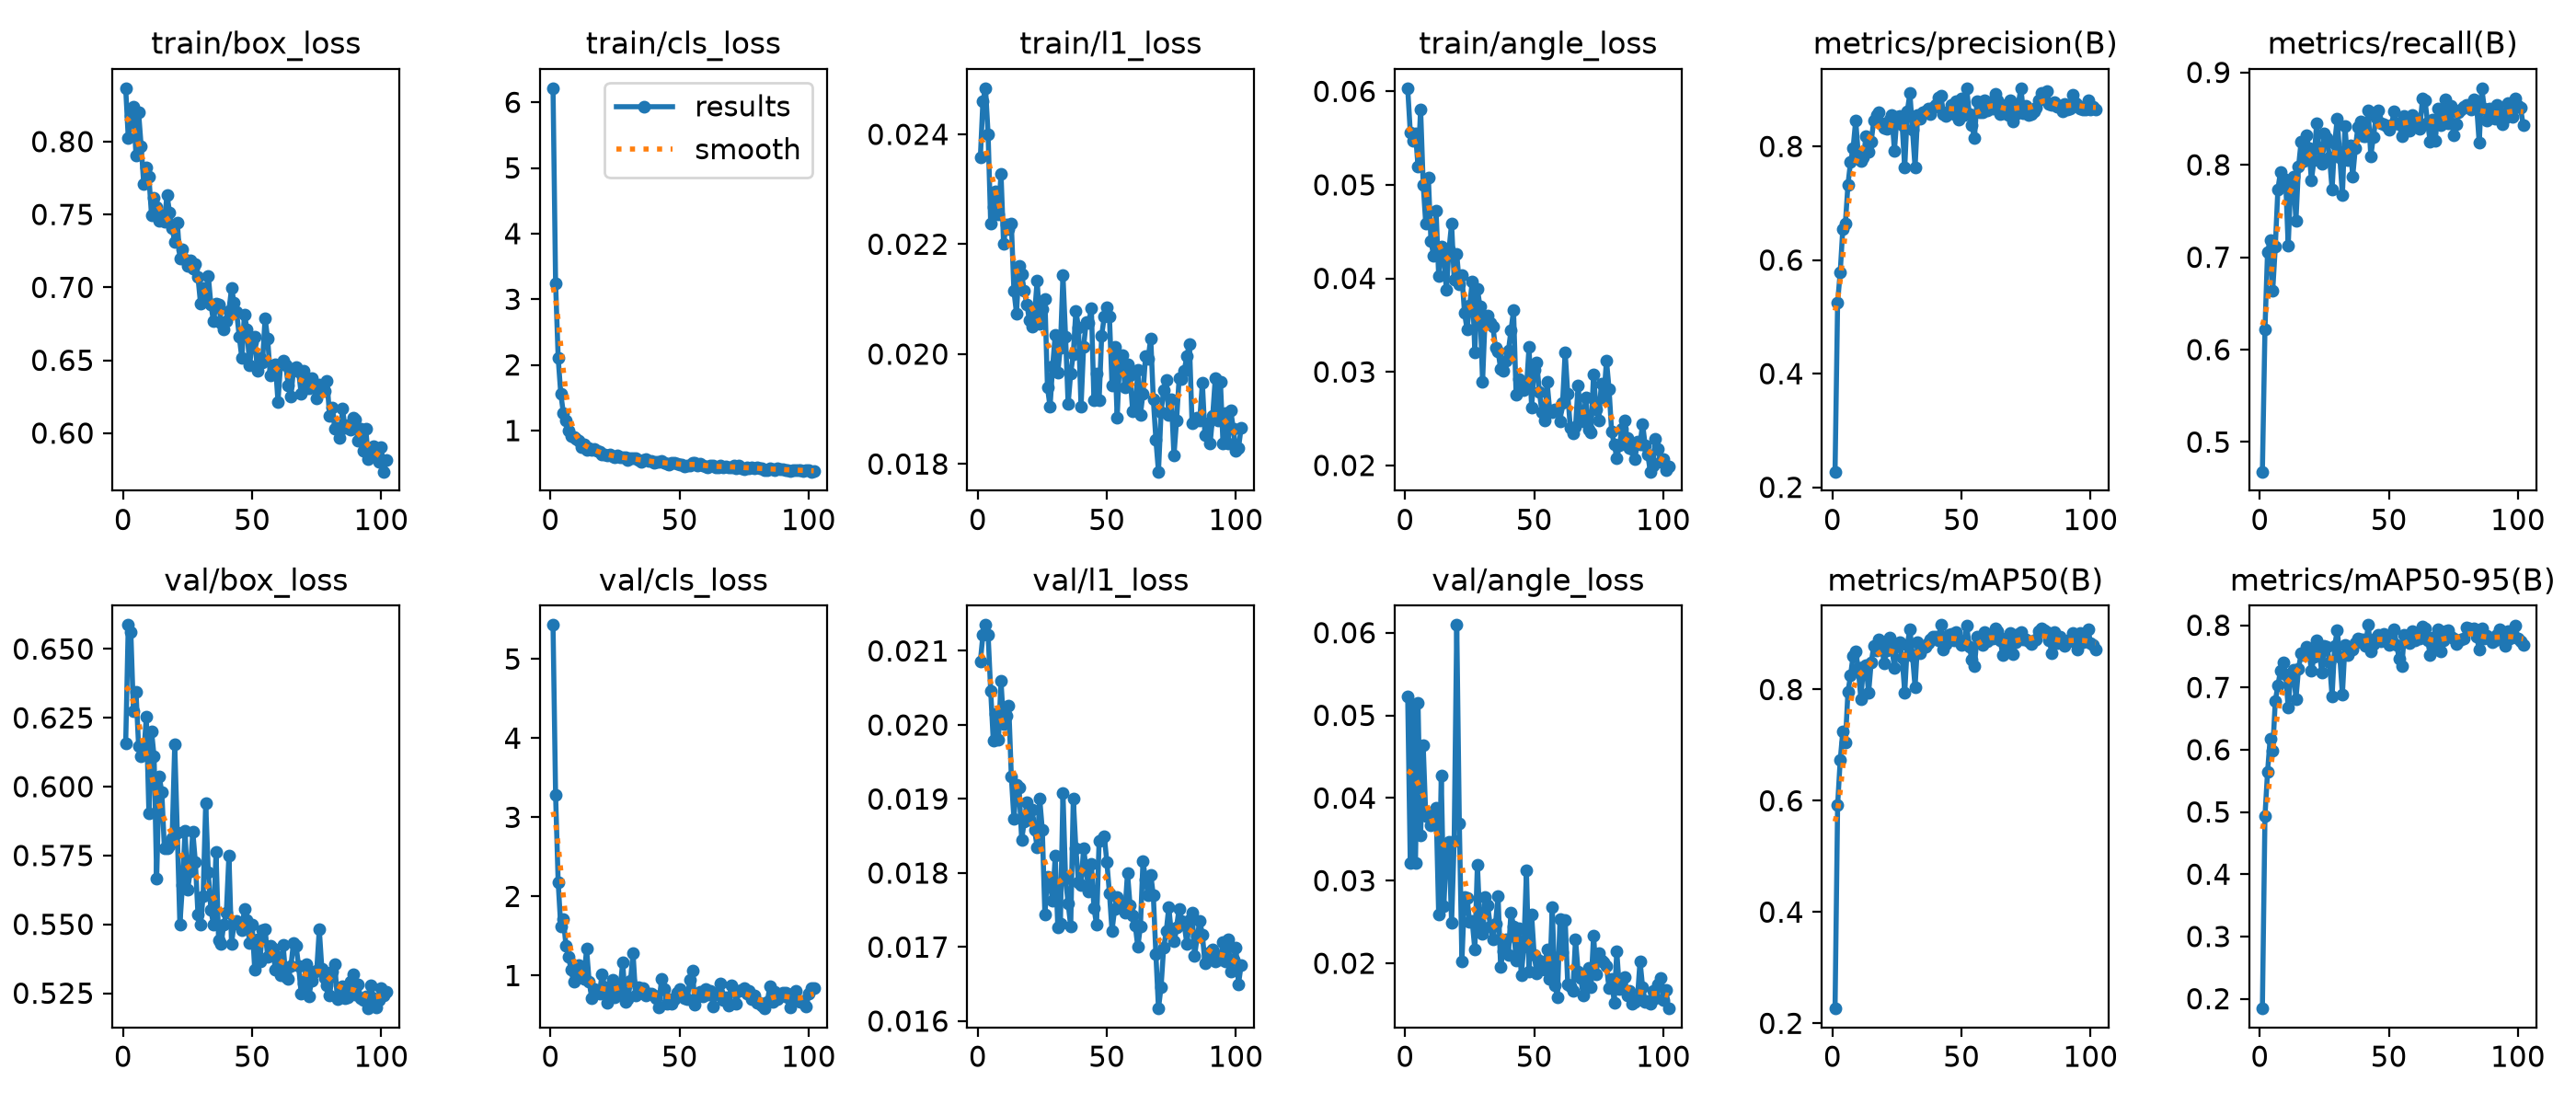
\includegraphics[width=\columnwidth]{fig_curves.png}
\caption{Training and validation curves for the medium-scale run. Best validation
fitness occurs at epoch 42 and is not challenged for the following 60 epochs, at
which point early stopping terminates the run. The last 60 epochs form a plateau, not
a degradation.}
\label{fig:curves}
\end{figure}

\subsection{Training cost and latency}
Per-epoch cost is 17.1~s (nano), 26.9~s (small) and 27.5~s (medium). The medium run
does not run faster per epoch than the small single-card run despite twice the
silicon: it is roughly twice the parameters and 3.3 times the FLOPs, so the second
card approximately pays for the extra depth rather than adding throughput, and the
per-step gradient all-reduce consumes part of what remains. The nano run is
loader-bound, with the GPU busy about half the time; sizing its batch to the model
would have halved its wall clock without changing the effective batch, since the
nominal batch is absorbed by gradient accumulation.

Inference at $1024$~px and batch 1 costs 4.0~ms for the small model and 9.5~ms for the
medium one, of which preprocessing is 1.1~ms and postprocessing 0.8~ms in the former
case. Postprocessing is cheap in absolute terms because suppression has been removed
from the pipeline; with suppression, cost would scale with the number of boxes and
would dominate on dense aprons. The medium model therefore costs 2.4 times the small
model's latency for $+0.025$ mAP@0.5, which is the central trade-off for deployment.

\begin{figure}[t]
\centering
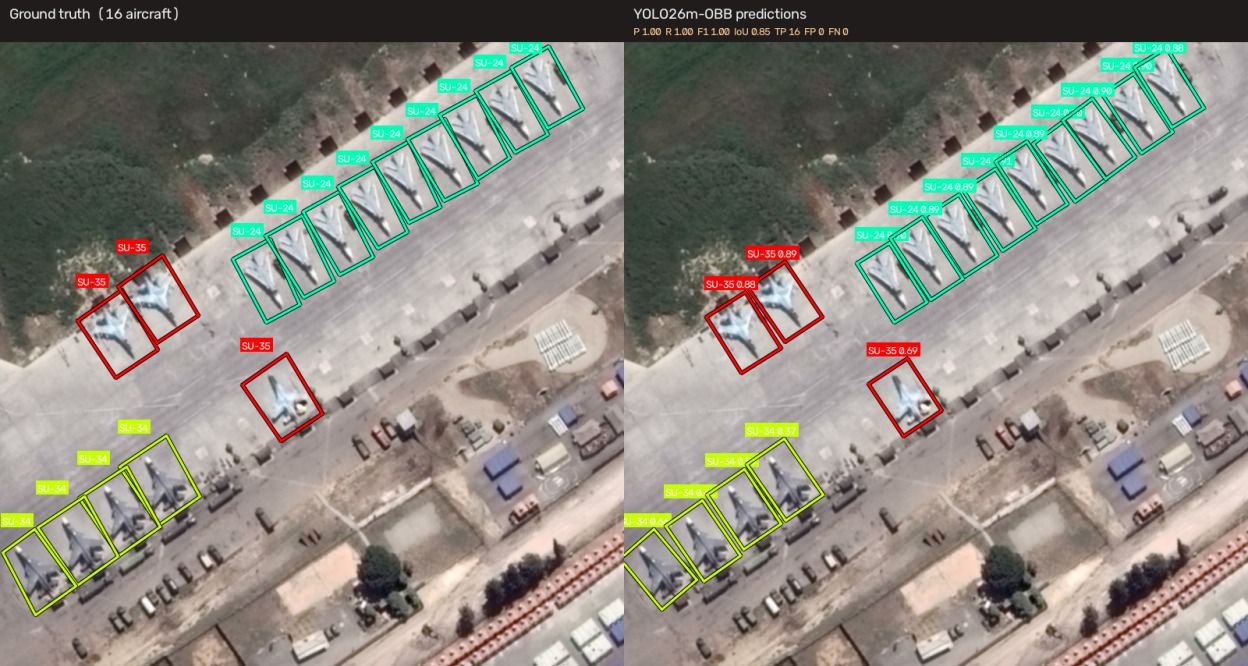
\includegraphics[width=\columnwidth]{fig_pred.jpg}
\caption{Validation predictions on a mixed Russian-fighter apron (ground truth left,
predictions right). Nine SU-24, four SU-34 and three SU-35 are detected with no false
positives and no misclassifications at IoU 0.5, illustrating the medium model's
behaviour on the classes where orientation and separation matter most.}
\label{fig:pred}
\end{figure}

\subsection{Qualitative behaviour}
Fig.~\ref{fig:pred} shows a typical dense result. Oriented boxes follow airframe
heading, so adjacent aircraft in a row remain separable with no suppression step.
Across the full validation split, predictions were scored class-aware against labels
at IoU 0.5: mean per-image F1 is 0.856, and 57.7\% of frames are error-free at that
threshold. The 111 frames with no true positive at all are dominated by the
precision-limited fighter classes discussed above.

\section{Limitations}
\label{sec:limits}

\emph{Numerics across devices.} Fixed seed and deterministic kernels do not give
bit-identical results across GPU counts: distributed training averages batch-norm
statistics across devices, and kernel selection differs. Fourth-decimal agreement
between the training loop and the standalone validation pass (0.9160/0.8003 versus
0.916/0.801) is the expected level of agreement, not a guarantee.

\emph{Latency provenance.} All timings are from the training GPU, not from an edge
device, and include no thermal or power constraint. They are useful for ranking the
scales against each other and should not be quoted as deployment figures.

\emph{Compute budget.} The ladder stops at the medium backbone because that is the
largest model trainable at $1024$~px with the resources available: the medium run
already needed two 48~GB accelerators at $16$ images per card, and the small model
exceeded 25~GB on a single card at the same resolution and total batch. Extending the
ladder to the large and extra-large variants of the family is therefore a question of
hardware rather than of patience. At this input resolution and batch size they exceed
what a pair of L40S cards can hold, and would need accelerators with substantially
more memory---an H200-class device (141~GB of HBM), or a multi-node cluster with
sharded or checkpointed training---plus proportionally more compute time and power.
The medium rung should be read as an accuracy ceiling for this setting, not as the
ceiling of the architecture family.

\section{Conclusion}
\label{sec:concl}

A single training recipe at $1024$~px with full rotation augmentation, applied to
three backbone scales of YOLO26-OBB on MAR20, produces a monotonic accuracy ladder
ending at mAP@0.5 of 0.916 and mAP@0.5:0.95 of 0.801, with a converged level of
0.889/0.779. Per-class analysis shows that the doubling from small to medium is
almost entirely a fighter-recall intervention: two classes gain 0.11 and 0.23 while
fifteen of the remaining eighteen move by 0.03 or less and the large airframes are saturated. The one class
that more capacity did not help, and slightly harmed in precision, is a twin-tail
planform that the sensor cannot separate from its siblings at this ground sample
distance.

Two conclusions follow for practice. First, aggregate mAP is an inadequate summary
for this benchmark, because the interesting dynamics are confined to four of twenty
classes and differ in kind between them. Second, the useful question when scaling a
detector is not how much accuracy a larger backbone buys but which error mode it
buys it from; here that mode was detection, and the identity mode remained.

Future work is in three directions: quantifying accuracy under FP16 and INT8
TensorRT on an 8~GB embedded module, where shared memory rather than compute is the
binding constraint; repeating the ladder across seeds to convert the two steps into
distributions; and attacking the identity-limited class with hard-negative mining
against the other twin-tail fighters or an upstream crop-and-reclassify stage. A
fourth rung at the large scale is the obvious extension and the one we cannot report
here: at $1024$~px it needs H200-class memory or multi-node training, so it belongs
to a cluster budget rather than a two-card one.

\section*{Acknowledgment}
The author thanks the maintainers of the MAR20 benchmark and of the Ultralytics
toolchain on which the experiments were built.

\begin{thebibliography}{99}

\bibitem{redmon2016}
J. Redmon, S. Divvala, R. Girshick, and A. Farhadi, ``You only look once: Unified,
real-time object detection,'' in \emph{Proc. IEEE Conf. Comput. Vis. Pattern
Recognit. (CVPR)}, 2016, pp. 779--788.

\bibitem{lin2017focal}
T.-Y. Lin, P. Goyal, R. Girshick, K. He, and P. Doll\'ar, ``Focal loss for dense
object detection,'' in \emph{Proc. IEEE Int. Conf. Comput. Vis. (ICCV)}, 2017,
pp. 2980--2988.

\bibitem{tian2019fcos}
Z. Tian, C. Shen, H. Chen, and T. He, ``FCOS: Fully convolutional one-stage object
detection,'' in \emph{Proc. IEEE Int. Conf. Comput. Vis. (ICCV)}, 2019, pp. 9627--9636.

\bibitem{zhou2019objects}
X. Zhou, D. Wang, and P. Kr\"ahenb\"uhl, ``Objects as points,'' \emph{arXiv preprint
arXiv:1904.07850}, 2019.

\bibitem{xia2018dota}
G.-S. Xia \emph{et al.}, ``DOTA: A large-scale dataset for object detection in aerial
images,'' in \emph{Proc. IEEE Conf. Comput. Vis. Pattern Recognit. (CVPR)}, 2018,
pp. 3974--3983.

\bibitem{ding2019roitransformer}
J. Ding, N. Xue, Y. Long, G.-S. Xia, and Q. Lu, ``Learning RoI transformer for
oriented object detection in aerial images,'' in \emph{Proc. IEEE Conf. Comput. Vis.
Pattern Recognit. (CVPR)}, 2019, pp. 2849--2858.

\bibitem{han2021redet}
J. Han, J. Ding, N. Xue, and G.-S. Xia, ``ReDet: A rotation-equivariant detector for
aerial object detection,'' in \emph{Proc. IEEE Conf. Comput. Vis. Pattern Recognit.
(CVPR)}, 2021, pp. 2786--2795.

\bibitem{yang2021r3det}
X. Yang, J. Yan, Z. Feng, and T. He, ``R3Det: Refined single-stage detector with
feature refinement for rotating object,'' in \emph{Proc. AAAI Conf. Artif. Intell.},
2021, pp. 3163--3171.

\bibitem{yu2021mar20}
W. Yu, X. Sun, K. Yang, Y. Rui, and H. Lin, ``MAR20: A benchmark for military
aircraft recognition in remote sensing images,'' \emph{J. Radars}, 2021.

\bibitem{tan2019efficientnet}
M. Tan and Q. Le, ``EfficientNet: Rethinking model scaling for convolutional neural
networks,'' in \emph{Proc. Int. Conf. Mach. Learn. (ICML)}, 2019, pp. 6105--6114.

\bibitem{huang2017speed}
J. Huang \emph{et al.}, ``Speed/accuracy trade-offs for modern convolutional object
detectors,'' in \emph{Proc. IEEE Conf. Comput. Vis. Pattern Recognit. (CVPR)}, 2017,
pp. 7310--7311.

\bibitem{ultralytics}
Ultralytics, ``YOLO26: Object detection and oriented bounding boxes,''
\emph{Ultralytics Documentation}, 2026. [Online].
Available: \url{https://docs.ultralytics.com}

\end{thebibliography}

\end{document}
